\documentclass[18pt, aspectratio=169]{beamer}
% \documentclass{etp-beamer-fancy}
\usepackage[utf8]{inputenc}
% \usepackage{templates/mytemplate}
\usepackage{templates/beamerthemekit}
\usepackage{graphicx}
\usepackage{microtype}
\usepackage{xcolor}
\usepackage{hyperref}
\usepackage{siunitx}
\usepackage{upgreek}
\usepackage{appendixnumberbeamer}

\title{MVA Track Quality Estimation for the Belle II Experiment}
\subtitle{DPG Frühjahrstagung 2019}
\author[Michael Eliachevitch]{Florian~Bernlochner, Nils~Braun,
  \textbullet{}Michael~Eliachevitch, Felix~Metzner}
\titleimage{tracks_wide}
\titlelogo{belle2-logo}
\institute{ETP -- KIT}
\date{27 March 2019}

\newcommand{\kitemph}[1]{\textcolor{kit-green100}{\bf{#1}}}

\begin{document}

\selectlanguage{english}
\begin{frame}
  \titlepage
\end{frame}
\begin{frame}
  \frametitle{The Belle II Detector}
  \begin{center}
    \includegraphics[width=.75\textwidth]{figures/belle2_detector_dpgaachen.pdf}
  \end{center}
\end{frame}
\begin{frame}[plain]
  \begin{center}
    \includegraphics[width=.8\textwidth]{figures/vertexdetector.jpg}
  \end{center}
\end{frame}
\begin{frame}
  \frametitle{Tracking at Belle II}
  \begin{columns}
    \begin{column}{0.5\textwidth}
      \begin{itemize}
      \item $\sim$11 tracks per $\Upupsilon(\text{4S})$ decay event, but\ldots
      \end{itemize}
      \begin{itemize}
      \item \textcolor{kit-red100}{Challenges}
        \begin{itemize}
        \item large beam-induced backgrounds
        \item low-momentum tracks
        \end{itemize}
      \end{itemize}
      \begin{itemize}
      \item \textcolor{kit-green100}{Solution}
        \begin{itemize}
        \item multiple subdetectors
        \item and respective tracking algorithms
        \end{itemize}
      \end{itemize}
    \end{column}
    \begin{column}{0.5\textwidth}
      \centering
      \includegraphics[width=0.7\textwidth]{figures/eplus_eminus_to_b_bar_diagram.pdf}\\
      \includegraphics[width=0.7\textwidth]{figures/first_y4s.jpg}
    \end{column}
  \end{columns}
\end{frame}
\begin{frame}
  \frametitle{Tracking algorithms at Belle II}
  \begin{columns}
    \begin{column}{0.53\textwidth}
      \begin{itemize}
      \item \kitemph{CDC standalone tracking}\\
        based on the global Legendre transform (extended Hough)
      \item \kitemph{SVD standalone tracking}\\
        uses a cellular automaton algorithm
      \item \kitemph{Combinatorial Kalman Filter (CKF)}\\
        extrapolate from existing tracks to attach tracks/hits in other subdetectors (e.g. PXD)
      \end{itemize}
    \end{column}
    \begin{column}{0.47\textwidth}
      \centering
      \includegraphics[width=\textwidth]{figures/full_track_finding_simplified.pdf}
    \end{column}
  \end{columns}
\end{frame}
\begin{frame}
  \frametitle{Need for a quality indicator}
  
\end{frame}
\begin{frame}
  \frametitle{Summary}
\end{frame}
\begin{frame}
  \frametitle{References and Further reading}
\end{frame}
\backupbegin
\end{document}

%%% Local Variables:
%%% coding: utf-8
%%% mode: LaTeX
%%% TeX-engine: default
%%% TeX-master: t
%%% fill-column: 100
%%% ispell-dictionary: "english"
%%% eval: (flyspell-mode 1)
%%% End: